\documentclass{article}\usepackage[]{graphicx}\usepackage[]{color}
%% maxwidth is the original width if it is less than linewidth
%% otherwise use linewidth (to make sure the graphics do not exceed the margin)
\makeatletter
\def\maxwidth{ %
  \ifdim\Gin@nat@width>\linewidth
    \linewidth
  \else
    \Gin@nat@width
  \fi
}
\makeatother

\definecolor{fgcolor}{rgb}{0.345, 0.345, 0.345}
\newcommand{\hlnum}[1]{\textcolor[rgb]{0.686,0.059,0.569}{#1}}%
\newcommand{\hlstr}[1]{\textcolor[rgb]{0.192,0.494,0.8}{#1}}%
\newcommand{\hlcom}[1]{\textcolor[rgb]{0.678,0.584,0.686}{\textit{#1}}}%
\newcommand{\hlopt}[1]{\textcolor[rgb]{0,0,0}{#1}}%
\newcommand{\hlstd}[1]{\textcolor[rgb]{0.345,0.345,0.345}{#1}}%
\newcommand{\hlkwa}[1]{\textcolor[rgb]{0.161,0.373,0.58}{\textbf{#1}}}%
\newcommand{\hlkwb}[1]{\textcolor[rgb]{0.69,0.353,0.396}{#1}}%
\newcommand{\hlkwc}[1]{\textcolor[rgb]{0.333,0.667,0.333}{#1}}%
\newcommand{\hlkwd}[1]{\textcolor[rgb]{0.737,0.353,0.396}{\textbf{#1}}}%
\let\hlipl\hlkwb

\usepackage{framed}
\makeatletter
\newenvironment{kframe}{%
 \def\at@end@of@kframe{}%
 \ifinner\ifhmode%
  \def\at@end@of@kframe{\end{minipage}}%
  \begin{minipage}{\columnwidth}%
 \fi\fi%
 \def\FrameCommand##1{\hskip\@totalleftmargin \hskip-\fboxsep
 \colorbox{shadecolor}{##1}\hskip-\fboxsep
     % There is no \\@totalrightmargin, so:
     \hskip-\linewidth \hskip-\@totalleftmargin \hskip\columnwidth}%
 \MakeFramed {\advance\hsize-\width
   \@totalleftmargin\z@ \linewidth\hsize
   \@setminipage}}%
 {\par\unskip\endMakeFramed%
 \at@end@of@kframe}
\makeatother

\definecolor{shadecolor}{rgb}{.97, .97, .97}
\definecolor{messagecolor}{rgb}{0, 0, 0}
\definecolor{warningcolor}{rgb}{1, 0, 1}
\definecolor{errorcolor}{rgb}{1, 0, 0}
\newenvironment{knitrout}{}{} % an empty environment to be redefined in TeX

\usepackage{alltt}
\usepackage[letterpaper, total={6in, 8in}]{geometry} %size of paper
\usepackage{indentfirst} %indent after section 
\usepackage{graphicx}
\usepackage{amsmath} %number figure based on subsection also
\numberwithin{figure}{subsection} %number figure based on subsection also
\numberwithin{table}{subsection} %number table based on subsection also
\usepackage{caption}
\captionsetup[figure]{labelfont=bf}
\captionsetup[table]{labelfont=bf,position=below}

\setlength{\parindent}{8ex}
\setlength{\parskip}{2em}
\renewcommand{\baselinestretch}{2.0}
\usepackage[skip=0pt]{caption}

%%%%%%%%%%%%%%%%%%%%%%%%%%%%%%%%%%%%%%%%%%%%%%%%%%%%%%%%%%
\IfFileExists{upquote.sty}{\usepackage{upquote}}{}
\begin{document}
%\SweaveOpts{concordance=TRUE}

\setcounter{section}{2} 
\setcounter{page}{8}

\section{Data}
\subsection{Sampling Procedure}

A young mouse muscle fiber cell was picked and then magnified to 166 different images by using Transmission Electron Microscope (TEM) (Figure~\ref{cell}). \\

\bigbreak
\begin{figure}[h!]
  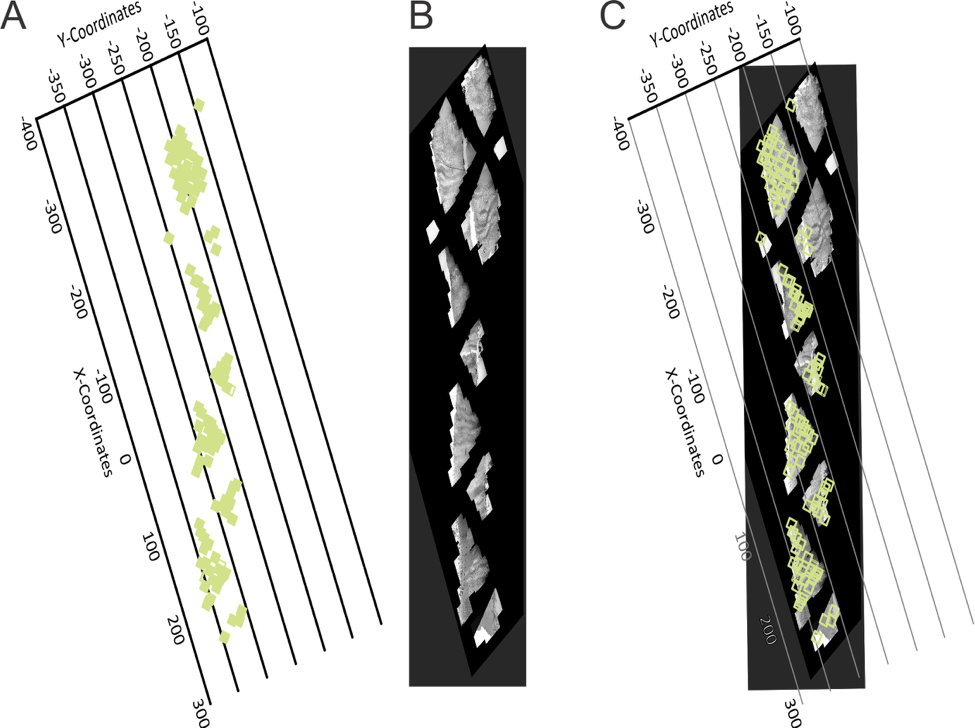
\includegraphics [width=11cm, scale=1.5]{cell.png}
  \centering
  \caption{A young mouse muscle fiber cell. These graphs is about how the 166 different images were defined on coordinate.} 
  \label{cell}
\end{figure}


For each location (Figure~\ref{location}), images were divided into two groups, Subsarcolemmal group and Interfibrillar group. In each group, one image was randomly picked and 20 mitochondria were chosen from the image. Due to high costs of labor on doing simple random sampling, mitochondria were chosen by other sampling method. A list of random two-dimensional coordinates was generated and the mitochondria were chosen as sample if their area in the photo included one or more generated coordinates (Figure~\ref{mitochondria}). \\

\bigbreak
\begin{figure}[h!]
  \centering
  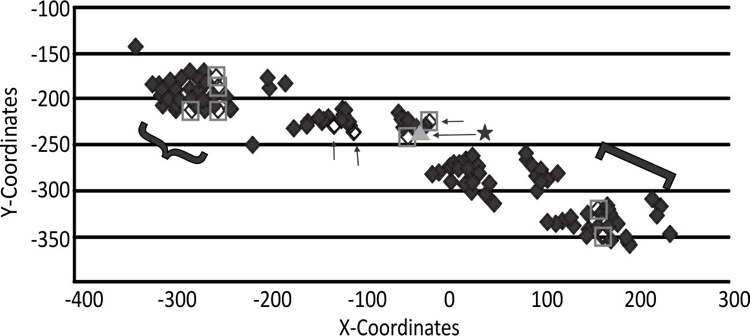
\includegraphics [width=11cm, scale=1.5]{location.png}
  \caption{Definition of Locations. Those falls in `` \{ '' are defined as being in Proximal end, in `` [ '' are being in Distal end, and the rest are being in Middle part.}
  \label{location}
\end{figure}

\bigbreak
\bigbreak

\begin{figure}[h!]
  \centering
  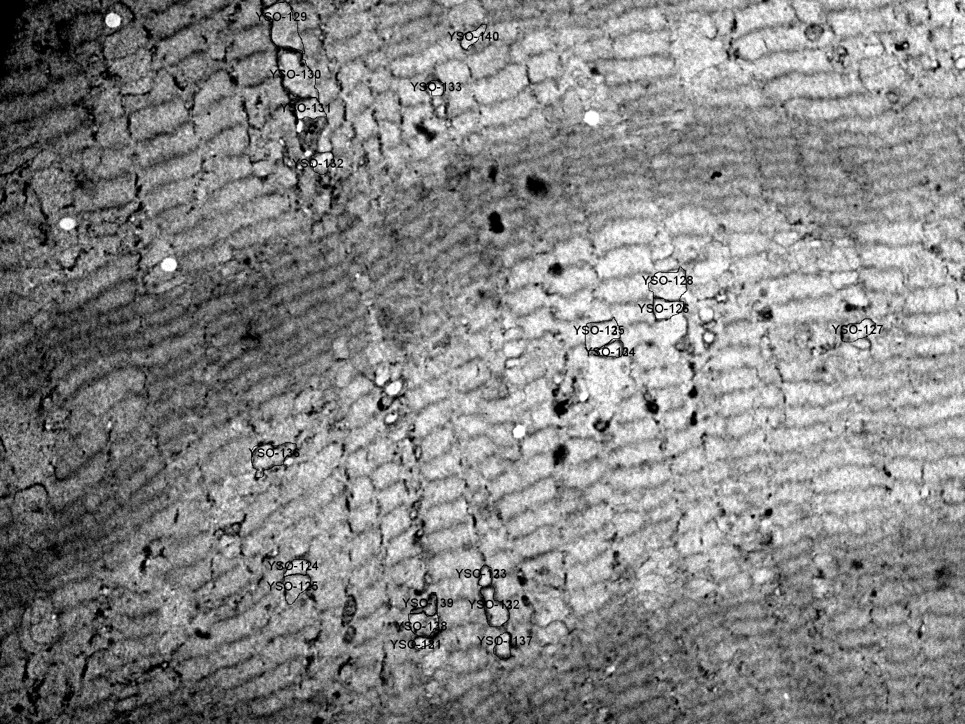
\includegraphics [width=11cm, scale=1.5]{mitochondria.png}
  \caption{A sample of Mitochondria}
  \label{mitochondria}
\end{figure}

\clearpage
\subsection{Data Description}
The following are the brief introduction about the attributions of each mitochondrion in this set of data. 

\setlength{\parskip}{0em}
\noindent\textbf{\underline{About locations and groups}}
\begin{itemize}
  \item Locations: \\
  The levels are Proximal end, Middle and Distal end.
  \item Groups: \\
  The levels are Subsarcolemmal and Interfibrillar groups. 
  \item Image ID number: \\
  From which image the mitochondrion is selected. 
  \item Mitochondrion ID number: \\
  The ID number of a mitochondrion in an image. 
\end{itemize}

\noindent\textbf{\underline{About the morphological properties}}
\begin{itemize}
  \item Area $({\mu m}^{2})$: \\
  The area occupied by a mitochondrion in an image. 
  \item Perimeter $(\mu m)$: \\
  The length of the boundary of a mitochondrion in an image. 
  \item Circularity: \\
  Circularity is equal to $\frac{4\pi Area}{{Perimeter}^{2}}$. Measuring the     resemblance of a mitochondrion to a circle. The range of circularity is     between 0 and 1.  1 means a perfect circle. 
  \item Aspect Ratio: \\
  Aspect Ratio is equal to $\frac{Length}{Width}$. If $AR\leq 2$, it is considered short; if $2<AR\leq 4$, intermediate; if $AR>4$, long.  
\end{itemize}

\setlength{\parskip}{2em}
\subsection{Descriptive Statistics}
To have a rough idea about how Properties of mitochondria differ over Locations in the set of data, the following four summary tables and eight figures provide information of descriptive statistics and distribution for each Property. 

As can be seen in Table~\ref{tab_area_pmd}, Figure~\ref{fig_area_pmd}, Table~\ref{tab_per_pmd}, Figure~\ref{fig_peri_pmd}, Table~\ref{tab_cir_pmd}, Figure~\ref{fig_cir_pmd}, the mitochondria at Distal part have the leftmost distributions of Area, Perimeter and Circularity; on the contrary, the ones at the Middle part have the rightmost distributions. This can be explained that generally Area, Perimeter and Circularity of mitochondria at Distal part are the smallest and the ones at the Middle part are the largest compared to the other two locations. Figure~\ref{fig_ar_pmd},  Table~\ref{tab_ar_pmd} show that different from other Properties, the mitochondria in Middle part generally have the lowest Aspect Ratio than ones in Proximal and Distal part. 

\newpage
%latex.default(table_A, rowname = NULL, file = "", label = "tab_area_pmd",     col.just = rep("c", 9), caption.loc = c("bottom"), caption = "Summary table for Area",     where = "!htbp", size = "footnotesize")%
\begin{table}[!htbp]
{\footnotesize
\begin{center}
\begin{tabular}{cccccccc}
\hline\hline
\multicolumn{1}{c}{PMD}&\multicolumn{1}{c}{Mean}&\multicolumn{1}{c}{Sd}&\multicolumn{1}{c}{min}&\multicolumn{1}{c}{Q1}&\multicolumn{1}{c}{Median}&\multicolumn{1}{c}{Q3}&\multicolumn{1}{c}{Max}\tabularnewline
\hline
Proximal&$2443.18$&$1309.09$&$845$&$1528.25$&$2056.5$&$3159.50$&$6740$\tabularnewline
Middle&$2957.50$&$1335.37$&$817$&$1831.00$&$2812.0$&$3848.25$&$6049$\tabularnewline
Distal&$1697.58$&$1262.37$&$335$&$~760.50$&$1423.5$&$2042.50$&$6283$\tabularnewline
\hline
\end{tabular}
\caption{Summary table for Area\label{tab_area_pmd}}\end{center}}
\end{table}

 \vspace{0.5cm}
%latex.default(table_A, rowname = NULL, file = "", label = "tab_per_pmd",     col.just = rep("c", 9), caption.loc = c("bottom"), caption = "Summary table for Perimeter",     where = "!htbp", size = "footnotesize")%
\begin{table}[!htbp]
{\footnotesize
\begin{center}
\begin{tabular}{cccccccc}
\hline\hline
\multicolumn{1}{c}{PMD}&\multicolumn{1}{c}{Mean}&\multicolumn{1}{c}{Sd}&\multicolumn{1}{c}{min}&\multicolumn{1}{c}{Q1}&\multicolumn{1}{c}{Median}&\multicolumn{1}{c}{Q3}&\multicolumn{1}{c}{Max}\tabularnewline
\hline
Proximal&$199.44$&$59.04$&$113.59$&$155.53$&$186.10$&$230.64$&$377.37$\tabularnewline
Middle&$214.27$&$47.31$&$116.81$&$179.25$&$210.82$&$248.78$&$310.46$\tabularnewline
Distal&$165.08$&$56.37$&$~79.27$&$130.99$&$155.29$&$191.17$&$324.78$\tabularnewline
\hline
\end{tabular}
\caption{Summary table for Perimeter\label{tab_per_pmd}}\end{center}}
\end{table}

 \vspace{0.5cm}

%latex.default(table_A, rowname = NULL, file = "", label = "tab_cir_pmd",     col.just = rep("c", 9), caption.loc = c("bottom"), caption = "Summary table for Circularity",     where = "!htbp", size = "footnotesize")%
\begin{table}[!htbp]
{\footnotesize
\begin{center}
\begin{tabular}{cccccccc}
\hline\hline
\multicolumn{1}{c}{PMD}&\multicolumn{1}{c}{Mean}&\multicolumn{1}{c}{Sd}&\multicolumn{1}{c}{min}&\multicolumn{1}{c}{Q1}&\multicolumn{1}{c}{Median}&\multicolumn{1}{c}{Q3}&\multicolumn{1}{c}{Max}\tabularnewline
\hline
Proximal&$0.74$&$0.11$&$0.52$&$0.67$&$0.78$&$0.82$&$0.90$\tabularnewline
Middle&$0.77$&$0.08$&$0.55$&$0.73$&$0.78$&$0.83$&$0.90$\tabularnewline
Distal&$0.70$&$0.10$&$0.35$&$0.64$&$0.73$&$0.77$&$0.84$\tabularnewline
\hline
\end{tabular}
\caption{Summary table for Circularity\label{tab_cir_pmd}}\end{center}}
\end{table}

 \vspace{0.5cm}

%latex.default(table_A, rowname = NULL, file = "", label = "tab_ar_pmd",     col.just = rep("c", 9), caption.loc = c("bottom"), caption = "Summary table for Aspect Ratio",     where = "!htbp", size = "footnotesize")%
\begin{table}[!htbp]
{\footnotesize
\begin{center}
\begin{tabular}{cccccccc}
\hline\hline
\multicolumn{1}{c}{PMD}&\multicolumn{1}{c}{Mean}&\multicolumn{1}{c}{Sd}&\multicolumn{1}{c}{min}&\multicolumn{1}{c}{Q1}&\multicolumn{1}{c}{Median}&\multicolumn{1}{c}{Q3}&\multicolumn{1}{c}{Max}\tabularnewline
\hline
Proximal&$1.53$&$0.52$&$1.05$&$1.16$&$1.35$&$1.73$&$3.64$\tabularnewline
Middle&$1.37$&$0.36$&$1.03$&$1.14$&$1.27$&$1.48$&$2.64$\tabularnewline
Distal&$1.53$&$0.41$&$1.10$&$1.24$&$1.40$&$1.72$&$2.92$\tabularnewline
\hline
\end{tabular}
\caption{Summary table for Aspect Ratio\label{tab_ar_pmd}}\end{center}}
\end{table}


\newpage
\begin{figure}[!htbp]
  \centering
\begin{knitrout}
\definecolor{shadecolor}{rgb}{0.969, 0.969, 0.969}\color{fgcolor}
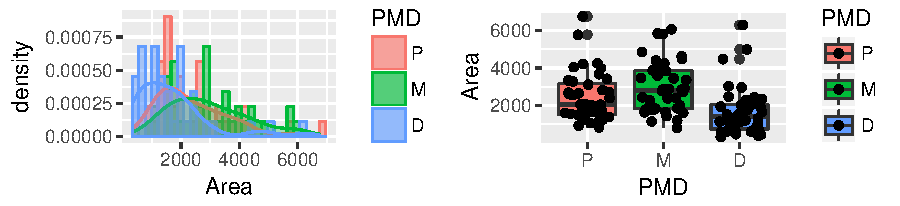
\includegraphics[width=\maxwidth]{figure/unnamed-chunk-5-1} 

\end{knitrout}
  \caption{Histogram and Boxplot for Area by Locations}
  \label{fig_area_pmd}
\end{figure}
\vspace{0.5cm}

\begin{figure}[!htbp]
  \centering
\begin{knitrout}
\definecolor{shadecolor}{rgb}{0.969, 0.969, 0.969}\color{fgcolor}
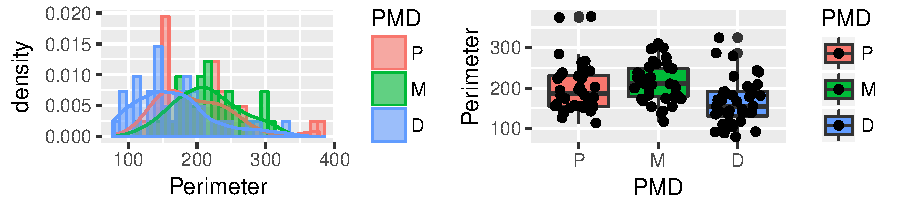
\includegraphics[width=\maxwidth]{figure/unnamed-chunk-6-1} 

\end{knitrout}
  \caption{Histogram and Boxplot for Perimeter by Locations}
  \label{fig_peri_pmd}
\end{figure}
\vspace{0.5cm}

\begin{figure}[!htbp]
  \centering
\begin{knitrout}
\definecolor{shadecolor}{rgb}{0.969, 0.969, 0.969}\color{fgcolor}
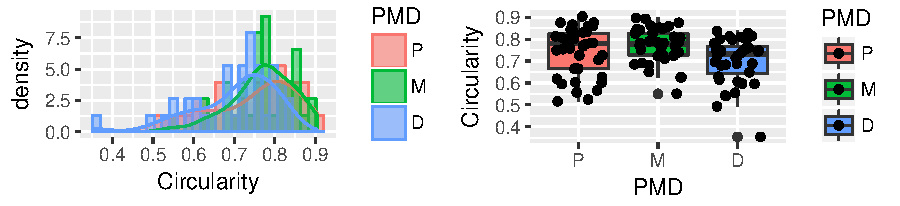
\includegraphics[width=\maxwidth]{figure/unnamed-chunk-7-1} 

\end{knitrout}
  \caption{Histogram and Boxplot for Circularity by Locations}
  \label{fig_cir_pmd}
\end{figure}
\vspace{0.5cm}

\begin{figure}[!htbp]
  \centering
\begin{knitrout}
\definecolor{shadecolor}{rgb}{0.969, 0.969, 0.969}\color{fgcolor}
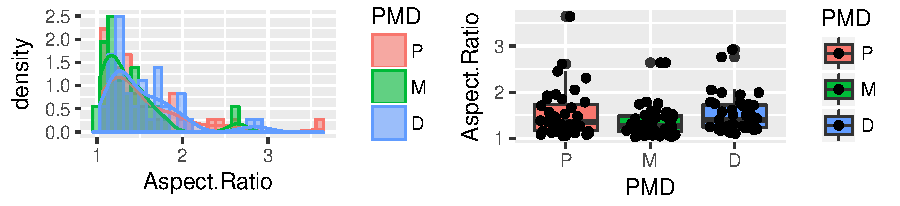
\includegraphics[width=\maxwidth]{figure/unnamed-chunk-8-1} 

\end{knitrout}
  \caption{Histogram and Boxplot for Aspect Ratio by Locations}
  \label{fig_ar_pmd}
\end{figure}
\end{document}
